% prelab3
\documentclass{IEEEtran}
\usepackage{booktabs}
\usepackage{graphicx}
\usepackage{fancyhdr}
\usepackage{framed}
\usepackage{siunitx}
\usepackage{amsmath}
\pagestyle{fancy}
\lhead{}
\chead{}
\rhead{}
\lfoot{}
\cfoot{}
\rfoot{\thepage}
\title{Prelab 3 First-Order Filters}
\author{Group 8: Muhan Li \and Man Sun \and Mingxiao An \\ EE233 Circuit Theory}
\IEEEaftertitletext{\centering \vspace{-10pt} \fontsize{11}{11}\textsc{Department of Electrical Engineering, University of Washington, Seattle, WA, 98195} \vspace{10pt}}
\begin{document}
	\maketitle
	\section{\textbf{Prelab\#1}}
	\begin{equation*}
		H(\mathbf{j}\omega) = \frac{V_{out}}{V_{in}} = -\frac{R_f}{R_s}
	\end{equation*}
	\phantom{ } As the result shows, the frequency response of the circuit is obviously a negative number, which means the amplifier inverts the positive and negative of the input voltage.\\
	\section{\textbf{Prelab\#2}}
	\begin{equation*}
		\mathrm{gain} = | H(\mathbf{j}\omega) | = -\frac{R_f}{R_s} = -47
	\end{equation*}
	\phantom{ } This means that we need to choose two resistors and one is 47 times in resistance of the other. From the lab kit, we choose a 47$ \si{k\Omega} $ resistor and a 1$ \si{k\Omega} $ resistor. Our schematic is shown in graph[\ref{fig:201}].
	
	\begin{figure}[!htbp]
		\centering
		\begin{framed}
			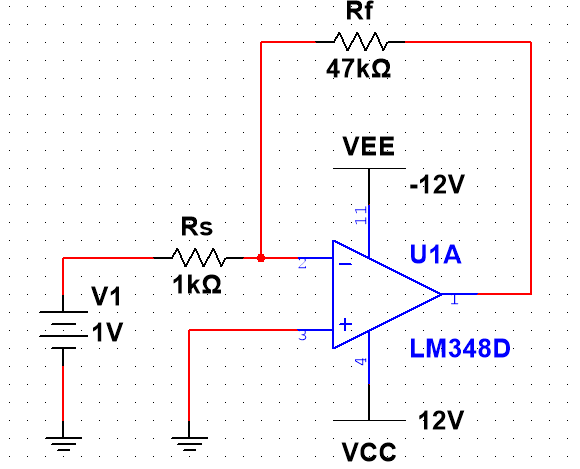
\includegraphics[width=\linewidth]{images/2_1.PNG}
			\caption{Schematic for inverting amplifier}
			\label{fig:201}
		\end{framed}
	\end{figure}

	\section{\textbf{Prelab\#3}}
	\subsection{the Matlab Bode plot}
	See figure[\ref{fig:301}]
	\begin{figure}[!htbp]
		\centering
		\begin{framed}
			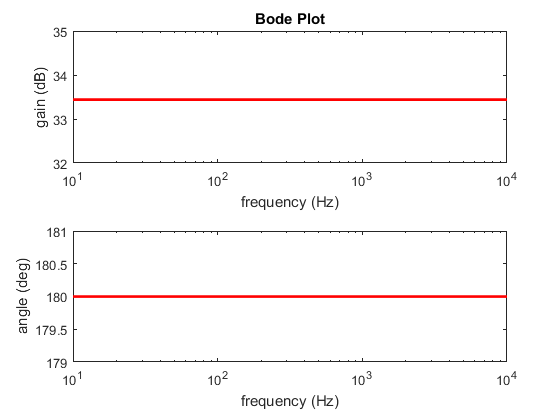
\includegraphics[width=\linewidth]{images/3_1.PNG}
			\caption{the Matlab Bode Plot for prelab \#3}
			\label{fig:301}
		\end{framed}
	\end{figure}
	\subsection{the SPICE Bode plot}
	\begin{figure}[!htbp]
		\centering
		\begin{framed}
			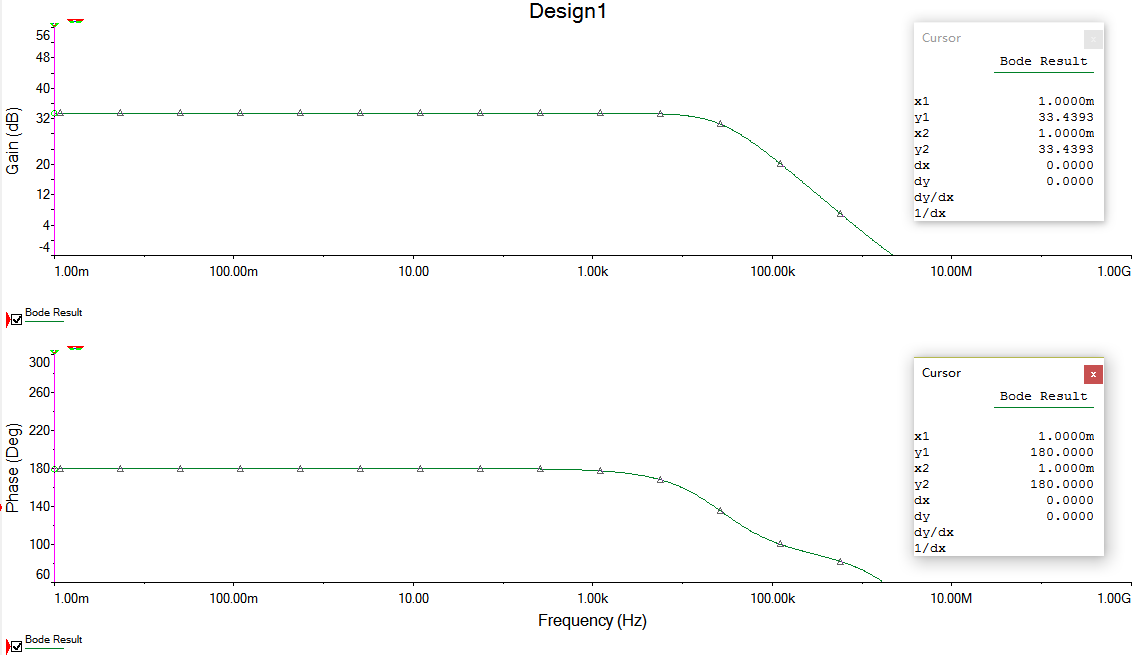
\includegraphics[width=\linewidth]{images/3_2.PNG}
			\caption{the SPICE Bode Plot for prelab \#3}
			\label{fig:302}
		\end{framed}
	\end{figure}
	\phantom{ } As the figure[\ref{fig:302}] shows, in low frequency range, the Bode plot simulated by SPICE is very close to the Bode plot simulated by matlab. However, in high frequency, the phase and the gain simulated by SPICE both falls down, which is not shown in the matlab plot. We think that SPICE simulates better than matlab, because of the falling tendency implied by the Bode plot from the datasheet. 
	\section{\textbf{Prelab\#4}}
	\begin{eqnarray*}
		\frac{V_{in}}{R_s} & = & \frac{V_{out}}{R_s + R_f}\\
		H(\mathbf{j}\omega) & = & \frac{V_{out}}{V_{in}} \quad = \quad \frac{R_s+R_f}{R_s}\\
	\end{eqnarray*}
	\phantom{ } We can see that the response is always a positive constant, so the output isn't inverted by the op amp, which is why it is known as a non-inverting amplifier.
	
	\section{\textbf{Prelab\#5}}
	\begin{eqnarray*}
		\frac{R_s+R_f}{R_s} & = & 48\\
		R_s & = & 1\si{k\Omega}\\
		R_f & = & 47\si{k\Omega}\\
	\end{eqnarray*}
	So we choose the same two resistors as in prelab \#2. The schematic graph is shown in figure[\ref{fig:501}].
	\begin{figure}[!htbp]
		\centering
		\begin{framed}
			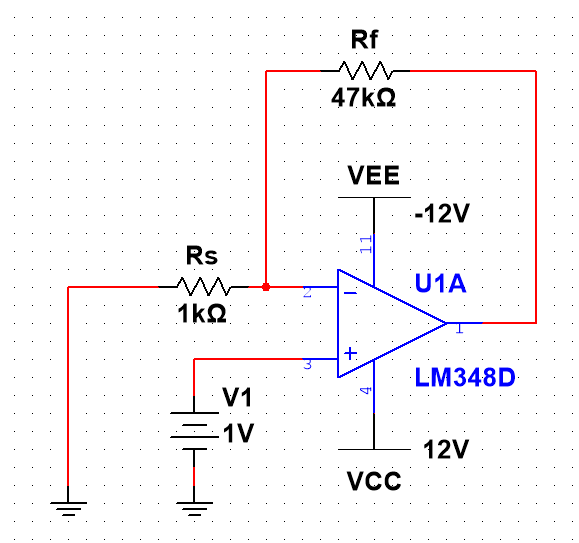
\includegraphics[width=\linewidth]{images/5_1.PNG}
			\caption{Schematic for non-inverting amplifier}
			\label{fig:501}
		\end{framed}
	\end{figure}

	\section{\textbf{Prelab\#6}}
	\subsection{the Matlab Bode Plot}
	See figure[\ref{fig:601}].
	\begin{figure}[!htbp]
		\centering
		\begin{framed}
			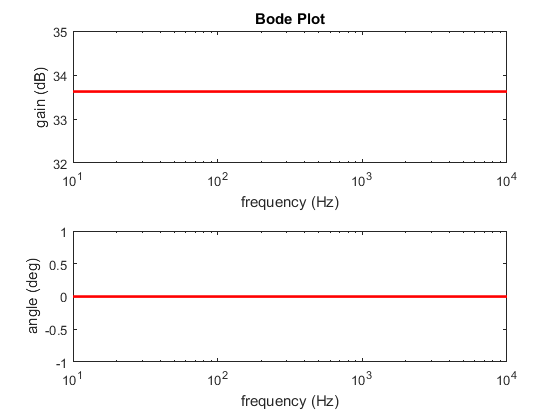
\includegraphics[width=\linewidth]{images/6.png}
			\caption{the Matlab Bode Plot for prelab \#6}
			\label{fig:601}
		\end{framed}
	\end{figure}

	\subsection{the SPICE Bode Plot}
	See figure[\ref{fig:602}].
	\begin{figure}[!htbp]
		\centering
		\begin{framed}
			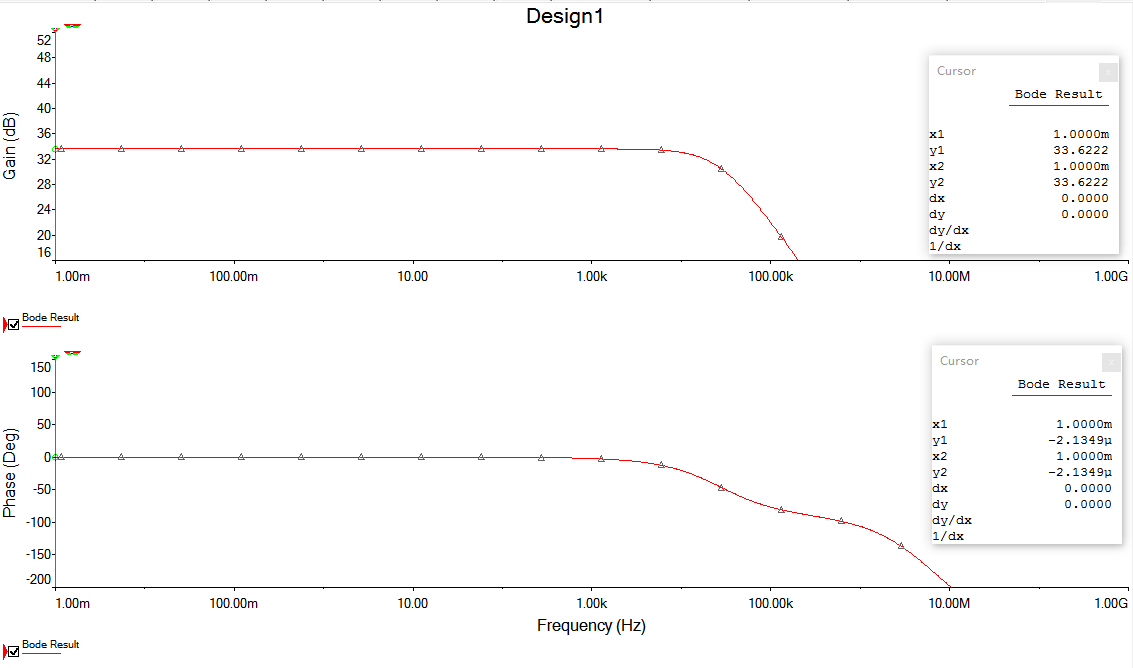
\includegraphics[width=\linewidth]{images/6_2.PNG}
			\caption{the SPICE Bode Plot for prelab \#6}
			\label{fig:602}
		\end{framed}
	\end{figure}
	\phantom{ } We can see that the difference appears in high frequency range. We think the reason for that is similar to the reason mentioned in prelab\#3.
	\section{\textbf{Prelab\#7}}
	\begin{eqnarray*}
		\frac{V_{in}}{R_s} & = & -\frac{V_{out}}{\frac{1}{\mathbf{j}\omega C}}\\
		H(\mathbf{j}\omega) & = & \frac{V_{out}}{V_{in}} \quad = \quad -\frac{1}{\mathbf{j}\omega CR_s}\\
	\end{eqnarray*}
	\phantom{ } We can see that if we do the Laplace inverse transformation on the frequency response, we get $ V_{out} = -\frac{1}{CR_s}\int V_{in} $, an integral of $ V_{in} $ with a factor of $ -\frac{1}{C R_s} $, which explains why the circuit performs the function of an integrator.
	\section{\textbf{Prelab\#8}}
	\begin{figure}[!htbp]
		\centering
		\begin{framed}
			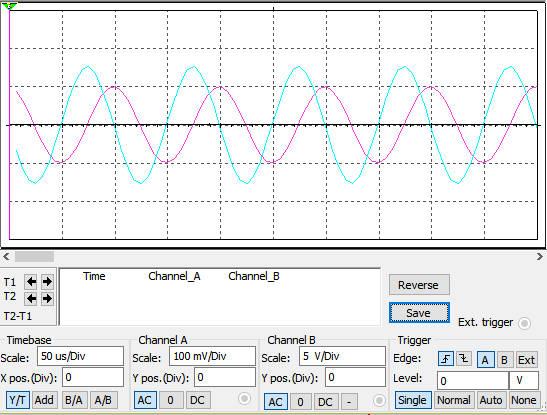
\includegraphics[width=\linewidth]{images/8_2.PNG}
			\caption{the SPICE waveforms for prelab \#8}
			\label{fig:801}
		\end{framed}
	\end{figure}
	\phantom{ } We used the oscilloscope to get the waveforms of input voltage and output voltage, because the real relationship between them appears after the output voltage reached a steady stage. From figure[\ref{fig:801}], we can see that output waveform is a cosine wave while the input is a sine wave. Also, the ratio of the two waveform's amplitudes is a constant. Thus, we confirm that the circuit functions as an integrator.
	\section{\textbf{Prelab\#9}}
	\subsection{the Matlab Bode Plot}
	See figure[\ref{fig:901}].
	\begin{figure}[!htbp]
		\centering
		\begin{framed}
			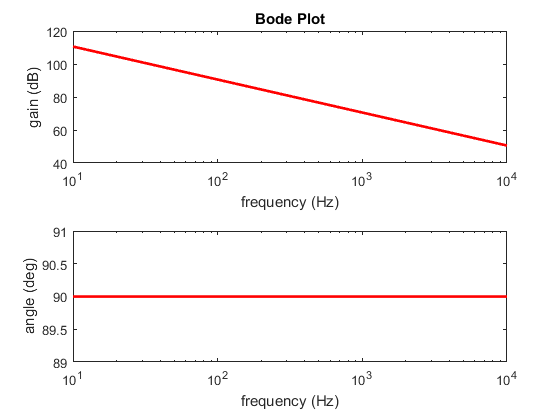
\includegraphics[width=\linewidth]{images/9.png}
			\caption{the Matlab Bode Plot for prelab \#9}
			\label{fig:901}
		\end{framed}
	\end{figure}
	\subsection{the SPICE Bode Plot}
	See figure[\ref{fig:902}].
	\begin{figure}[!htbp]
		\centering
		\begin{framed}
			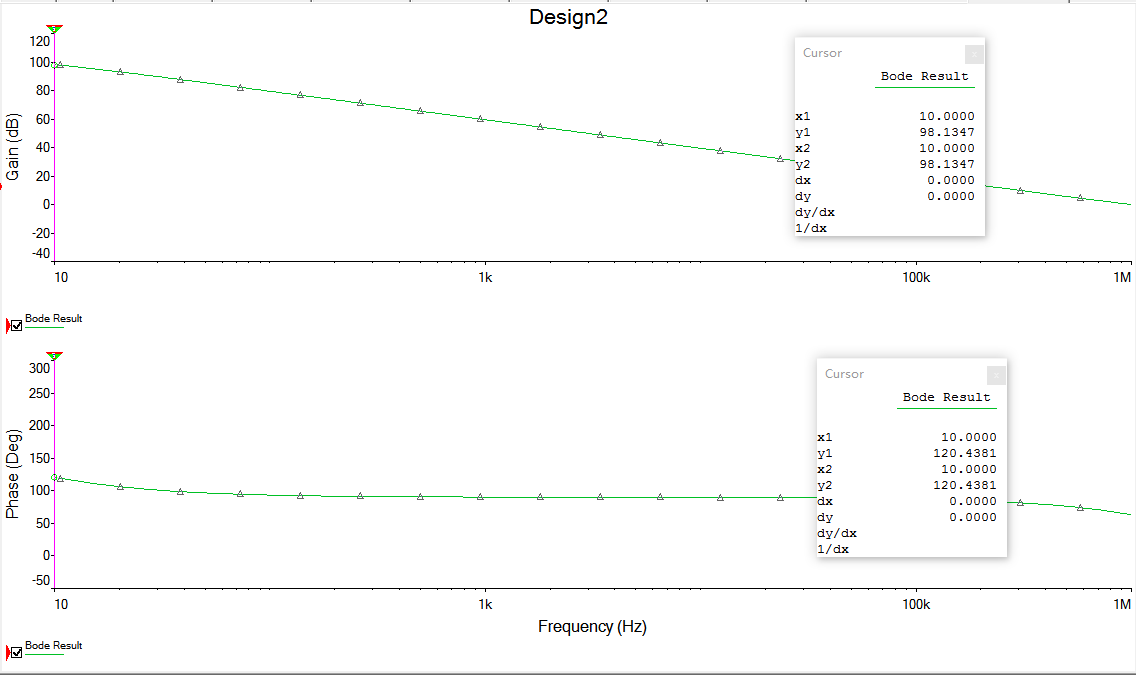
\includegraphics[width=\linewidth]{images/9_2.PNG}
			\caption{the SPICE Bode Plot for prelab \#9}
			\label{fig:902}
		\end{framed}
	\end{figure}

	\phantom{ } We can see from figure[\ref{fig:901},\ref{fig:902}] that the two graphs simulated by matlab and SPICE are very close. 
	\section{\textbf{Prelab\#10}}
	\subsection{the frequency response}
	\begin{eqnarray*}
		\frac{V_{in}}{R_s} & = & -\frac{V_{out}}{\frac{1}{\mathbf{j}\omega C}} - \frac{V_{out}}{R_f}\\
		H(\mathbf{j}\omega) & = & \frac{V_{out}}{V_{in}} \quad = \quad -\frac{R_f}{\mathbf{j}\omega CR_sR_f + R_s}\\
	\end{eqnarray*}
	\subsection{the magnitude of gain and Matlab Bode Plot}
	\begin{eqnarray*}
		\mathrm{gain} = |H(\mathbf{j}\omega)| = \frac{R_f}{\sqrt{(\omega C R_s R_f)^2 + R_s^2}}
	\end{eqnarray*}

	See figure[\ref{fig:1001}] for Matlab Bode plot.
	\begin{figure}[!htbp]
		\centering
		\begin{framed}
			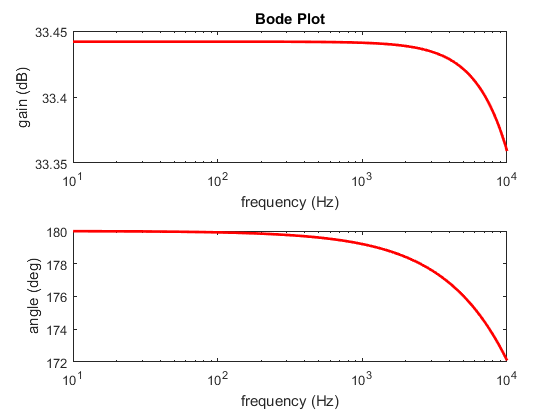
\includegraphics[width=\linewidth]{images/10.png}
			\caption{the Matlab Bode Plot for prelab \#10}
			\label{fig:1001}
		\end{framed}
	\end{figure}
	\section{\textbf{Prelab\#11}}
	\subsection{explanation at low frequency}
	\phantom{ } When $ \omega \to 0 $, the part $ (\omega C R_S R_f)^2 $ in the square root in denominator of the expression of gain also approaches to 0, which implies that the gain of this circuit approaches to $ \frac{R_f}{R_s} $, which is the same as the gain of an amplifier with constant gain. Also, we can see from the circuit schematic that if we take the capacitor(behave like unconnected in low frequency) away, the whole circuit is the same as an inverting amplifier. In low frequency, both the gain and the phase of two graphs are close. But in high frequency, when the frequency is not close to $ 0\si{\hertz} $, the gain and frequency in this circuit falls while those in inverting amplifier stay the same. 
	\subsection{explanation at high frequency}
	\phantom{ } When $ \omega \gg \frac{1}{R_fC} $, we can say that $ \omega CR_sR_f \gg R_s $, which means that the part $ R_s $ in the square root in the denominator of the expression of the gain can be ignored. So we can say when $ \omega \gg \frac{1}{R_fC} $, $ \mathrm{gain} \to \frac{1}{\omega CR_SR_f} $, which is the same as the gain if a simple integrator at high frequencies.
	\subsection{the function of $ R_f $}
	\phantom{ } Without a shunt resistor $ R_f $, like the circuit in prelab\#9, the gain of the integrator will be very high at low frequencies, which may result in high noise amplification at low frequencies. Also, high gain (also known as drift) at low frequencies may exceed the limitation of the op-amp.
	\section{\textbf{Prelab\#12}}
	\subsection{SPICE simulation}
	We simulated the circuit and get the Bode Plot in figure[\ref{fig:1201}].\\
	\begin{figure}[!htbp]
		\centering
		\begin{framed}
			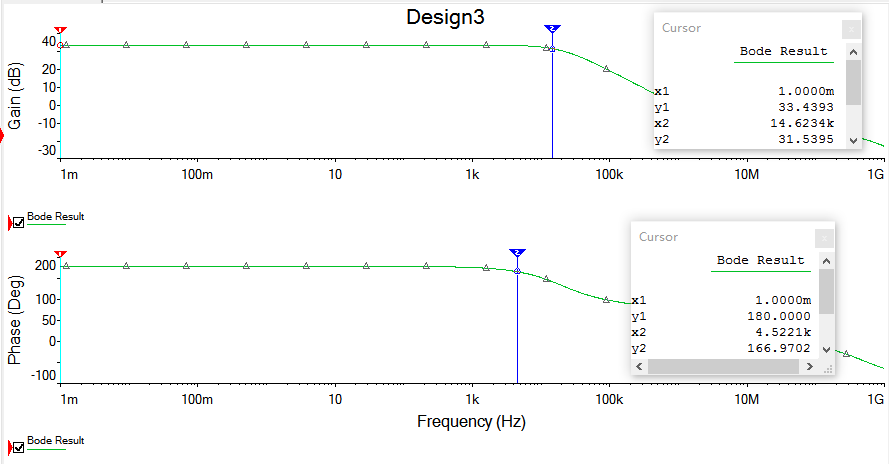
\includegraphics[width=\linewidth]{images/12_1.PNG}
			\caption{the SPICE Bode Plot for prelab \#12}
			\label{fig:1201}
		\end{framed}
	\end{figure}
	\phantom{ } As the figure shows, if the input signal has a low frequency, the expected gain is 33.4393dB, and if the input signal has a high frequency, the expected gain will fall when the frequency goes higher.
	\subsection{comment}
	\phantom{ } This circuit has a stable and high gain at lower frequencies, so it is a low-pass filter. It has a more stable performance and is able to lower the noise as well as amplify the signal. However, non-inverting amplifiers and inverting amplifiers only provides a constant gain without selectivity, which means that they cannot lower noise. So this circuit is a better choice for preamplifier (the first amplifier in a signal processing procedure).
	\section{\textbf{Prelab\#13}}
	\begin{eqnarray*}
		\frac{V_{in}}{\frac{1}{\mathbf{j}\omega C}} & + & \frac{V_{out}}{R_f}  =  0\\
		H(\mathbf{j}\omega) & = & \frac{V_{out}}{V_{in}}  =  -\mathbf{j}\omega CR_f
	\end{eqnarray*}
	\phantom{ } We can see that if we do Laplace inverse transformation on $ -\mathbf{j}\omega CR_f $, we can get a differentiation expression $ -CR_f\frac{\mathrm{d}}{\mathrm{d}t} $, which implies that this circuit functions as a differentiator.
	\section{\textbf{Prelab\#14}}
	\begin{figure}[!htbp]
		\centering
		\begin{framed}
			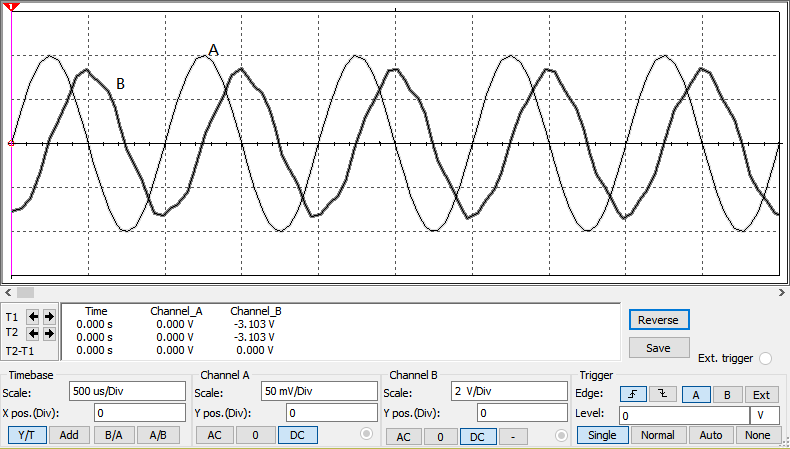
\includegraphics[width=\linewidth]{images/14_1.PNG}
			\caption{the SPICE waveforms Plot for prelab \#14}
			\label{fig:1401}
		\end{framed}
	\end{figure}
	\phantom{ } We can see from figure[\ref{fig:1401}], where input signal is channel A, and output signal is channel B, that the two waveforms have a phase difference of 90 degrees and have a shape close to sine waves. Also, the ratio of the two waveforms' amplitudes stays the same. These features imply the function of the circuit as a differentiator.
	\section{\textbf{Prelab\#15}}
	\subsection{the Matlab Bode Plot}
	See figure[\ref{fig:1501}].
	\begin{figure}[!htbp]
		\centering
		\begin{framed}
			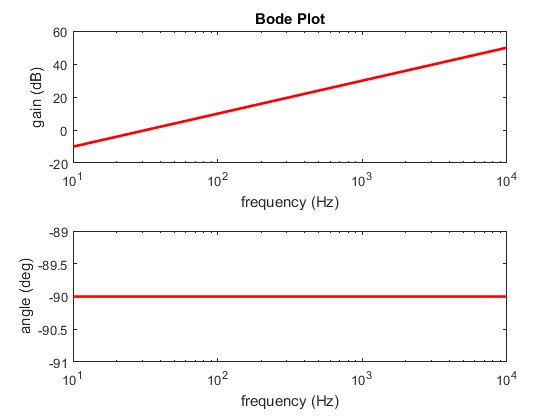
\includegraphics[width=\linewidth]{images/15.png}
			\caption{the Matlab Bode Plot for prelab \#15}
			\label{fig:1501}
		\end{framed}
	\end{figure}
	\subsection{the SPICE Bode Plot}
	See figure[\ref{fig:1502}].
	\begin{figure}[!htbp]
		\centering
		\begin{framed}
			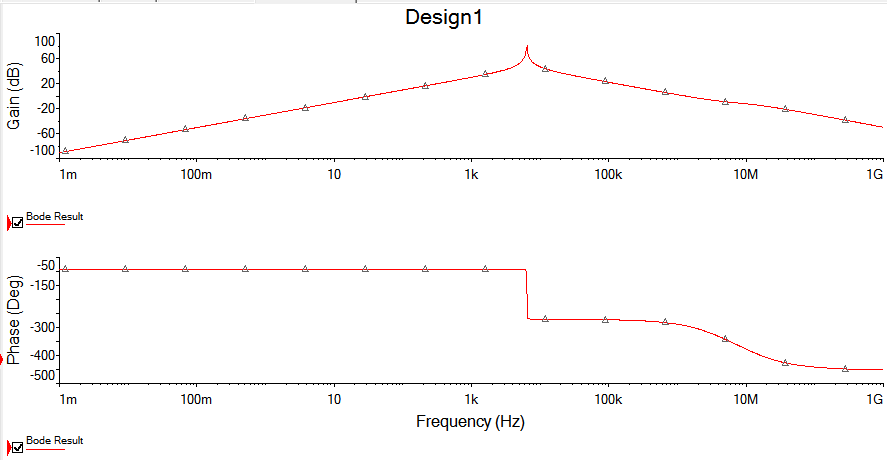
\includegraphics[width=\linewidth]{images/15_1.PNG}
			\caption{the SPICE Bode Plot for prelab \#15}
			\label{fig:1502}
		\end{framed}
	\end{figure}
\end{document}